\documentclass[border=10pt]{standalone}
\usepackage{pgfplots}
\usepackage{siunitx}
\pgfplotsset{width=7cm,compat=1.8}
\usepgfplotslibrary{polar}
\pgfplotsset{mypolarplot/.style={%
  clip=false, % needed for double line (last \addplot command)
  domain=0:360, % plot full cycle
  samples=300, % number of samples; can be locally adjusted
  grid=both, % display major and minor grids
  major grid style={black}, 
  minor x tick num=3, % 3 minor x ticks between majors
  minor y tick num=1, % 1 minor y tick between majors
  xtick={0,90,...,359},
  xticklabels={%
    $\theta = \ang{90}$,
    $\theta = \ang{0}$,
    $\theta = \ang{270}$,
    $\theta = \ang{180}$
  },
  yticklabel style={anchor=east}, % move label position
}}
\begin{document}
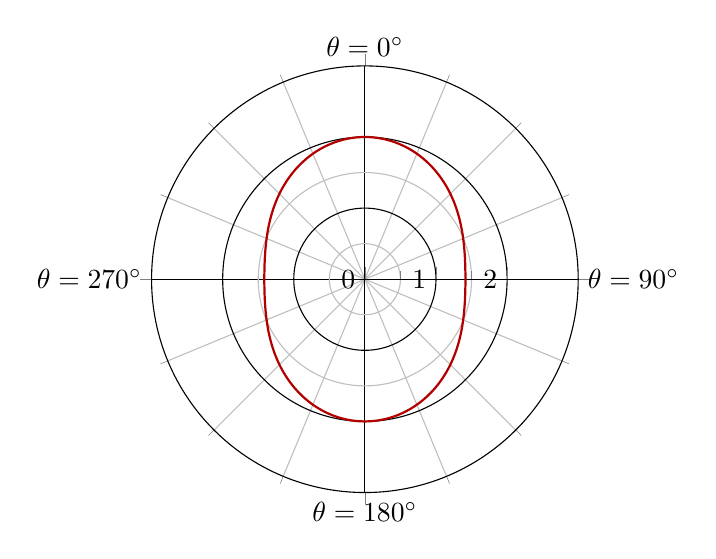
\begin{tikzpicture}

    \pgfmathsetmacro{\alpha}{0}
      \pgfmathsetmacro{\d}{1/4}
    \begin{polaraxis}[%
        ymax=3,
        ytick={0,1,2},
        mypolarplot,
      ]
        \addplot[mark=none,thick,red!70!black] 
        {2*cos(45*cos(\x)+\alpha)}; 
; % there is likely a better way to do this
      \end{polaraxis}
\end{tikzpicture}
\end{document}